\newpage
\section{Literature Review}
In this section, the related work are discussed in the following dimensions:
\begin{enumerate}
    \item Exact Bayesian inference methods.
    \item Several encoding schemes that can reduce the computation of probability of the evidence for a Bayesian Network into a Weighted model counting problem. 
    \item Exisiting model counting tools.
\end{enumerate}
    \subsection{Bayesian inference methods}
        \subsubsection{Variable Elimination}
        Variable Elimination is a Exact inference method propsed in \cite{Varelimination}. The idea is to exploit the structure by eliminating the non-observed and non-queried variables once at a time.\\
        
       \noindent A Factor is a function from a tuple of random variables to a number, denoted by $f(X_{1}, X_{2}, ... , X_{j})$, it denotes a distribution over $\{X_{1}, .., X_{j}\}$. 
        \begin{itemize}
            \item  By assigning some of (or all of) the variables in a factor, new factors can be made out of an existing factor. For example: $f(X_{1} = v_{1}, X_{2}, ..., X_{j})$ is a factor of $\{X_{2}, ... , X_{j}\}$ when $v_{1}$ is assigned to $X_{1}$.
            \item A variable can be signed out. Consider the $X_{1}$ over domain $\{v_{1}, .. ,v_{m}\}$, the variable $X_{1}$ can be summed out with the formula below: $$\Sigma_{i= 1}^{m}f(X1 = v_{i}, X_{2}, ..., X_{j})$$
            \item Factors can be multiplied. Consider two factors $f_{1}(X_{1}, X_{2}, X_{3})$ and $f_{2}(X_{1}, X_{4}, X_{5})$ which they both have $X_{2}$ in common. A new factor is defined below: $$(f_{1} \times f_{2})(X_{1}, .. X_{5}) = f_{1}(X_{1}, X_{2}, X_{3}) \times f_{2}(X_{1}, X_{4}, X_{5}) $$
        \end{itemize}
        
        \noindent Given variables over a Bayesian Network $X_{1}, ... , X_{m}$, the factor $P(Z, Y_{1}=v_{1}, ... , Y_{j}= v_{j})$ can be computed by summing out $Z_{1}, ..., Z_{k} =  \frac{\{X_{1}, ... X_{n}\}}{Z, Y_{1}, ..., Y_{j}}$.\\
        
        \noindent Given the factors $P(X_{i}|iX_{i})$ and chain rule, $P(X_{1}, ..., X_{n})$ can be written as: $\Pi_{i = 1}^{n} P(X_{i}|pX_{i})$. So we have:
        $$P(Z, Y_{1}=v_{1}, ... , Y_{j}= v_{j}) = \Sigma_{Z_{k}}.. \Sigma_{Z_{1}} \Pi P(X_{i}|pX{i})_{Y_{1} = v1, .. Y_{j} = v_{j}}$$
        
       
        \noindent To sum up, the Variable elimination algorithm is to repeat
        \begin{enumerate}
            \item choose a variable to eliminate.
            \item push in its sum as far as possible.
            \item Compute the sum to result in a new factor.
        \end{enumerate}
        \newpage
        \noindent \textbf{Complexity of Variable Elimination}\\
        
        \noindent The time and space complexities of Bayesian inference with Variable Elimination algorithm depends on the size of the largest intermediate factor. It is a NP-hard problem to choose the elimination order that minimize the complexity.\\
        
        \noindent The Variable Elimination is also query sensitive, that is the query variables should be specified in advance. Each time we run a diffenerent query, we must re-run the entire algorithm.
        
        \subsubsection{Junction tree}
        Junction tree algorithm, or sometimes called Joint tree algorithm is another exact Bayesian inference algorithm introduced in \cite{junctree}. This algorithm generalize Variable Elimination to deal with the query sensitive problem. It can execute a large number of queried simultaneously.\\
        
        \noindent \textbf{Define a junction tree:}\\

        \noindent The cluster graph T is a junction tree is it satisfy the following three properties:
        
        \begin{enumerate}
            \item \textbf{Single connectivity:} A cluster graph satisfy singly connectivity if there is one and only one path connecting between each cluster.
            \item \textbf{Covering:} A cluster graph satisfy covering if got each clique A of G, there is some cluster C such that A $\subseteq$ C.
            \item \textbf{Running intersection:}  A cluster graph satisfy  running intersection if for each pair of clusters B and C that both contain \textit{x}, the cluster between the unique path connecting B and C also contains \textit{x}.
        \end{enumerate}
        
        \noindent To build a junction tree, first choose an order of nodes and perform Variable elimination to obtain elimination cliques, then build the complete cluster graph over the maximum elimination cliques, after that, weight the edges and compute the maximum weight juntion tree.
        Figure \ref{fig:bayesjunc} shows a Bayesian network and its corresponding junction tree with the assignment of the factors.\\
        
        \begin{figure}
            \centering
            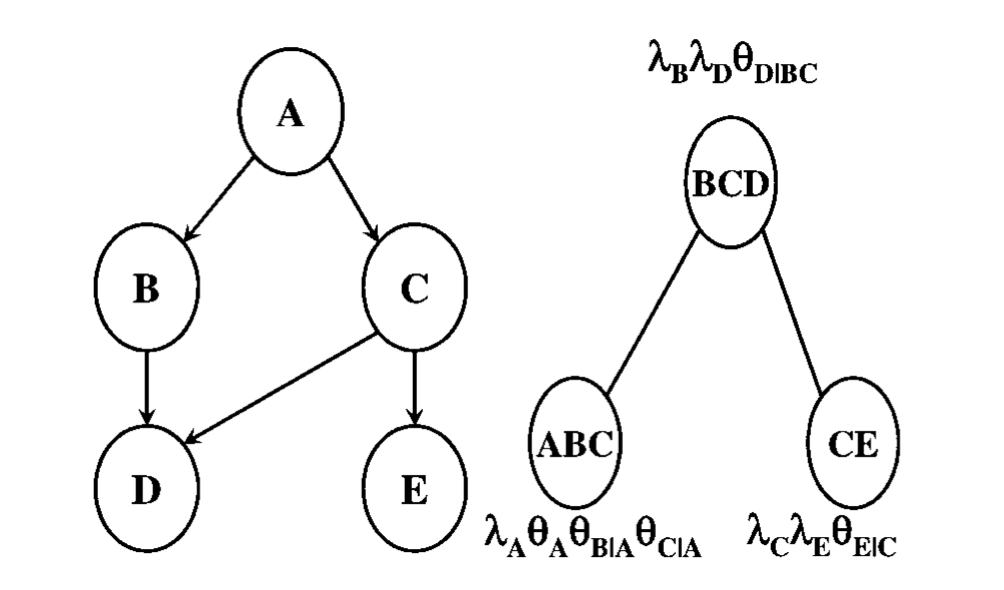
\includegraphics[width = 0.6\textwidth, height = 0.3\textwidth]{pic/bayesandjunctree.png}
            \caption{Left A Bayesian network, Right: its corresponding junction tree}
            \label{fig:bayesjunc}
        \end{figure}
        
        \noindent \textbf{Complexety of junction tree algorithm}\\
        
        \noindent Junction tree algorithm can be viewed as a decent way of performing Variable elimination. Different elimination orders will lead to different junction trees and finding the junction tree that have the smallest cluster is a NP-hard problem.\\
        
        \noindent The time and space complexity is dominated by the size of the largest cluster in the junction tree. The complexity with tabular density Bayesian Networks is \textbf{exponential} in the size of the largest cluster.
        
        
        \subsubsection{Weighted model Counting}
        To perform Bayesian Inference with Weighted model counting, the Bayesian networks are represented as multi\-linear functions and encoded into Conjunctive Normal Forms (CNF) and feed the CNFs are feed into Model Counters. The section below describes several encoding schemes to perform Weighted model counting method, and also review several existing model counters.
    
    \subsection{Encoding Bayed to CNF}
        \subsubsection{Full encoding}
            The first encoding algorithm that we called Full encoding, was proposed in \cite{enc1}, In this section, we will first define the logical variables and introduce the steps to generate the clauses.\\
            
            \noindent \textbf{Generating CNFs}
            \newline
            Given a Bayesian Network, two types of variables are generated.
            Define the variables generated from Node \textbf{\textit{X}} as Indicator Variables.
            For a node \textbf{\textit{X}} in Bayesian Network \textbf{N}, let $\lambda_x$ define the indicator variable. 
            Define the variables generated form Node \textbf{\textit{X}} and its parents \textbf{Y} = {$Y_{1}$, ... $Y_{n}$} as Parameter Variables.
            For a node \textbf{\textit{X}} in Bayesian Network \textbf{N}, let $\theta_{X|Y}$ denotes the parameter variable.\\
            
            \noindent \textbf{Obtaining indicator clauses \textsc{I}:}\\
            For each node \textit{X} in a Bayesian Network with probability \{$x_{1}$,... ,$x_{n}$\} $\in$ \textit{X}, the following clauses are generated:
            % Indicator Clauses and Parameter Clauses
            \begin{equation}\label{fullenc_ic1}
                \lambda_{x_{1}} \vee ... \vee \lambda_{x_{n}}
            \end{equation}
            
            \begin{equation}\label{eq:fullenc_ic2}
                \neg\lambda_{x_{i}} \vee \neg\lambda_{x_{j}}, \;\;\; \mbox{for each i $\neq$ j}
            \end{equation}
            According to the commutation of logic OR, $R \vee Q$ $\Longleftrightarrow$ $Q \vee R$, to avoid redundant clauses, \ref{eq:fullenc_ic2} can be simplified as :
            \begin{equation}\label{fullenc_ic3}
                \neg\lambda_{x_{i}} \vee \neg\lambda_{x_{j}}, \;\;\; \mbox{for each i $<$ j}
            \end{equation}
            
            % parameter clauses
            \noindent \textbf{Obtaining parameter clauses \textsc{P}:}\\
            For each node \textbf{\textit{X}} in a Bayesian Network and its parents \textbf{\textit{Y}}, the following clauses are generated:
            \begin{equation}\label{fullenc_pc1}
                \lambda_{x_{i}} \wedge \lambda_{y_{1}} \wedge... \wedge \lambda_{y_{m}} \leftrightarrow \theta_{x_{i}|y_{1}..y{m}}
            \end{equation}
            
            % parameter clauses
           \noindent The following equation is the equivalent of \ref{fullenc_pc1} written in the way that meet the requirement of CNF.
            \begin{equation}\label{fullenc_IP}
                \neg\lambda_{x_{i}} \vee \neg\lambda_{y_{1}} \vee... \vee \neg\lambda_{y_{m}} \vee \theta_{x_{i}|y_{1}..y_{m}}
            \end{equation}
            \begin{equation}\label{fullenc_PI}
                \neg\theta_{x_{i}|y_{1}..y_{m}} \vee \lambda_{x_{i}},\\ \;\;
                \neg\theta_{x_{i}|y_{1}..y_{m}} \vee \lambda_{y_{j}} \;\; \mbox{ j = 1, ..., m}
            \end{equation}
            An example is given below. Consider a Bayesian network 'Asia', figure \ref{fig:asia-tub} shows two of the nodes 'asia' and 'tub'.
            
            \begin{figure}[h]
            \centering
            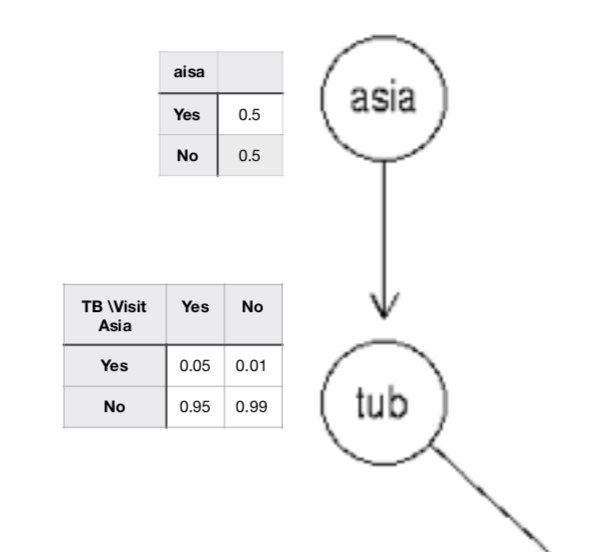
\includegraphics[width=0.25\textwidth]{pic/asia-tub.png}
            \caption{Two nodes from Asia Bayesian network}
            \label{fig:asia-tub}
            \end{figure}
            %% Here should be the example with BN asia
            \newpage
            \begin{multicols}{2}
            [
            \noindent The following clauses are generated for Node aisa and Node TB:
            ]
            \noindent \textbf{Node asia} = \{$Visit\_asia_{yes}$, $Visit\_asia_{no}$\}\\
            \newline
            \textbf{Indicator clauses:}\\
            $\lambda_{asia_{Y}} \vee \lambda_{asia_{N}}$\\
            $\neg \lambda_{asia_{Y}} \vee \neg\lambda_{asia_{N}}$\\
            \newline
            \textbf{Parameter clauses:}\\
            $\lambda_{asia_{Y}} \rightarrow \theta_{asia_{Y}}$\\
            $\theta_{asia_{Y}} \rightarrow \lambda_{asia_{Y}}$\\
            %%% fen ge xian %%%
            
            \columnbreak
            \noindent \textbf{Node TB} = $\{Tubercolosis_{yes}, Tubercolosis_{no}\}$:\\
            \newline
            \textbf{Indicator clauses:}\\
            $\lambda_{TB_{Y}} \vee \lambda_{TB_{N}}$\\
            $\neg \lambda_{TB_{Y}} \vee \neg\lambda_{TB_{N}}$\\
            \newline
            \textbf{Parameter clauses:}\\
            $\lambda_{TB_{Y}} \wedge \lambda_{asia_{Y}}\rightarrow \theta_{TB_{Y}|asia_{Y}}$\\
            $\theta_{TB_{Y}|asia_{Y}} \rightarrow \lambda_{TB_{Y}}$\\
            $\theta_{TB_{Y}|asia_{Y}} \rightarrow \lambda_{asia_{Y}}$\\
            $\lambda_{TB_{N}} \wedge \lambda_{asia_{Y}} \rightarrow \theta_{TB_{N}|asia_{Y}}$\\
            $\theta_{TB_{N}|asia_{Y}} \rightarrow \lambda_{TB_{N}}$\\
            $\theta_{TB_{N}|asia_{Y}} \rightarrow \lambda_{asia_{Y}}$\\
            \end{multicols}
            
        \subsubsection{Simplified Full encoding}
        The second encoding scheme, which we refer to as Simplified Full encoding, is the simplification of the previous encoding scheme presented in \cite{enc1}. The main simplification is to capture the deterministic of Bayesian Networks.\\
        
        \noindent \textbf{Nodes with cardinality = 2}\\
        Now consider the node with cardinality 2. Take an Example in asia network, in figure \ref{fig:asia-tub} node \textit{asia} has two possibilty \textit{Yes} and \textit{No}, so according to \ref{fullenc_ic1}, we have $\lambda_{Visitaisa_{yes}} \vee \lambda_{Visitaisa_{no}}$ and this will always be 1, and the same apply for $\neg\lambda_{Visitaisa_{yes}} \vee \neg\lambda_{Visitaisa_{no}}$ \\
        \newline
        \noindent \textit{Simplification step 1:} If the cardinality of a node in a Bayesian Network is 2, ommit the clause in formula \ref{fullenc_ic1} and formula \ref{fullenc_ic3} in \textit{3.2.1 Full Encoding}.
        \newline
        
        \noindent \textbf{Encoding deterministic:}\\
        Now take a closer look at the values in each CPT, the deterministic can be captured.\\
        
        \noindent \textit{Simplification step 2:} When the parameter variable $\theta_{x_{i}|y_{1}..y_{m}}$ = 0, the parameter clause \textbf{P} described by \ref{fullenc_pc1} can be written as a single clause: $$\neg\lambda_{x_{i}} \vee \neg\lambda_{y_{1}} \vee... \vee \neg\lambda_{y_{m}}.$$
        
        \noindent \cite{enc1} gives the explanation of this step: If network variable $\theta_{x_{i}|y_{1}..y_{m}}$ = 0, then each term with indicator variables $\lambda_{x}, \lambda_{y_{1}}, \lambda_{y_{2}}, ..., \lambda_{y_{m}}$ is multiplied by 0 in the multi\-linear function, thus those clauses have no contributions to he multi\-linear function.\\
        \newline
        \noindent \textit{Simplification step 3:} When the parameter variable $\theta_{x_{i}|y_{1}..y_{m}}$ = 1, the parameter can be omitted and the clause \ref{fullenc_PI} and \ref{fullenc_IP} can be eliminated from the encoding.\\
        
        \noindent The explanation is given in section 4.2 in \cite{enc1} 
        Since $\theta_{x_{i}|y_{1}..y_{m}}$ = 1, terms with includes $\lambda_{x_{i}}, \lambda_{y_{1}}, ..., \lambda_{y_{m}}$ are multiplied by 1. 
        Consider the example with a network Either in Asia Bayesian network in Figure \ref{fig:either01}
        
        \begin{figure}[h]
            \centering
            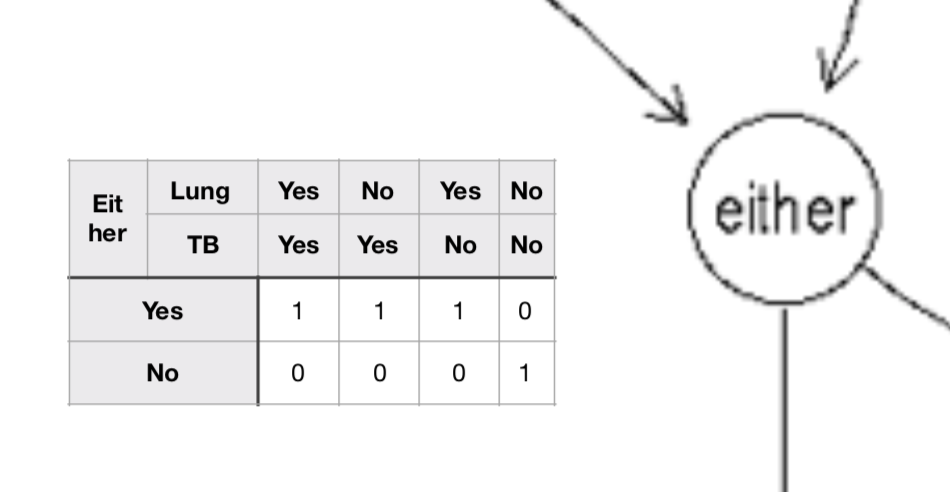
\includegraphics[width=0.4\textwidth]{pic/either01s.png}
            \caption{Node \textit{Either} from Asia Bayesian network}
            \label{fig:either01}
        \end{figure}
        
        \noindent After simplification, the clause generated by node \textit{Either}:\\
        \begin{center}
            $\neg \lambda_{Either_{yes}} \vee \neg \lambda_{Lung_{no}} \vee \neg  \lambda_{TB_{no}} $\\
            $\neg \lambda_{Either_{No}} \vee \neg \lambda_{Lung_{yes}} \vee \neg \lambda_{TB_{yes}}$\\
            $\neg \lambda_{Either_{No}} \vee \neg \lambda_{Lung_{No}} \vee \neg  \lambda_{TB_{yes}}$\\
            $\neg  \lambda_{Either_{No}} \vee \neg  \lambda_{Lung_{yes}} \vee \neg  \lambda_{TB_{no}}$
        \end{center}
        
        \noindent In paper \cite{enc2} proved that this simplification will lead to large reduction in the CNF sizes, the results are further discusses in Section 7.3 Encoding deterministic.\\
        
        \noindent \textbf{Weights assigning rules}:\\
        
        \noindent For each CNF literal, we need to assign a weight. These are the rules for assigning weights
        \begin{itemize}
            \item For both positive and negative indicator variables, assign weights to 1.
            \item For negative parameter variables, assign weights to 1.
            \item For positive parameter variables, assign weights that is the same as the parameter values in the CPTs.
        \end{itemize}
       
        For example, consider Nodes Aisa and Tub in Figure \ref{fig:asia-tub} and the clauses they generate. 
        \begin{center}
            $Weight(\theta_{asia_{Y}}) = 0.5$\\
            $Weight(\theta_{asia_{N}}) = 0.5$\\
            $Weight(\theta_{TB_{Y}}|Asia_{Y}) = 0.05$\\
            $Weight(\theta_{TB_{Y}}|Asia_{N}) = 0.01$\\
            $Weight(\theta_{TB_{N}}|Asia_{Y}) = 0.95$\\
            $Weight(\theta_{TB_{N}}|Asia_{N}) = 0.99$\\
        \end{center}
        The weight of the rest of the literals equals to 1. \\
        
        \noindent Now for each model, the weight of one model equals the product of all positive parameter variables. 
        $$\textbf{\textbf{W}} = \prod_{i = 0}^{n} Weight(\theta_{X_{n}}) $$
        The process to answer specific queries is to change the weight of variables with contradicting subscript to the indicators to 0.
        
        
        \subsubsection{Improved Encoding}
        The third Encoding Scheme, which we refer to as Improved Encoding, was introduced in \cite{enc2} based on the Simplified Full encoding scheme.
        The idea was to use less clauses and variables to encode the CPT by encoding equal parameters. A key observation of the CPT is that using the Improved Full Encoding, no two parameter variables generated from the same CPT can be set as TRUE simultaneously, since their network instantiations are not consistent. \cite{enc2} proposed that within a CPT, if there are multiple \textbf{non-extreme} variables that has the same value, instead of generating new variables each time, we can use one logic variable to represent the parameter values.\\
        
        \noindent \textbf{Obtaining indicator clauses \textsc{I}:}\\
        For each node \textit{X} in a Bayesian Network with probability \{$x_{1}$,... ,$x_{n}$\} $\in$ \textit{X}, the following clauses are generated:
        \begin{equation}\label{Improvedenc_ic}
            \lambda_{x_{1}} \vee ... \vee \lambda_{x_{n}}
        \end{equation}
        This step is the same as the Full encoding.\\

        \noindent \textbf{Obtaining Parameter clauses \textsc{P}:}\\
        For each node \textbf{\textit{X}} in a Bayesian Network and its corresponding CPT:
        \begin{itemize}
            \item For \textbf{extreme parameter values} in the CPT, parameter variables are generated as the same way as the Simplification of  Full encoding.
            \item For each \textbf{non-extreme value} \textit{v}, we generate one parameter variable $\theta_{v}$.\\
        \textbf{Problem Raised:} Following the full encoding scheme, assume the following part from Node C with parent nodes A and B in a Bayesian network:
        %\begin{center}
        \begin{multicols}{2}
        [
        The following parameter clauses are generated
        ]
        
        \begin{center}
        \vspace{10mm}
            \begin{tabular}{ c c c c } 
            \hline
            C & A & B & P\\
            \hline
            \hline
            $C_1$ & $A_1$ & $B_1$ & 0.2\\
            $C_2$ & $A_2$ & $B_2$ & 0.2\\
            \hline
            \end{tabular}\\ 
        \end{center} 
        \columnbreak
            
        $\lambda_{a_{1}} \wedge \lambda_{b_{1}} \wedge \lambda_{c_{1}} \rightarrow \theta_{0.2}$\\
        $ \theta_{0.2} \rightarrow \lambda_{a_{1}} \wedge \lambda_{b_{1}} \wedge \lambda_{c_{1}}$\\
        $\lambda_{a_{2}} \wedge \lambda_{b_{2}} \wedge \lambda_{c_{2}} \rightarrow \theta_{0.2}$\\
        $ \theta_{0.2} \rightarrow \lambda_{a_{2}} \wedge \lambda_{b_{2}} \wedge \lambda_{c_{2}}$\\
        \end{multicols}
        
        %\end{center}
        For the value 0.2 in this table, $\theta_{0.2}$ is used for the parameter variable, we got $ \theta_{0.2} \rightarrow \lambda_{a_{1}} \wedge \lambda_{b_{1}} \wedge \lambda_{c_{1}}$ and $ \theta_{0.2} \rightarrow \lambda_{a_{2}} \wedge \lambda_{b_{2}} \wedge \lambda_{c_{2}}$ in the clauses. The $\theta_{0.2}$ implies incompatible configurations of the variables\cite{enc2}.  \\
        
        \textbf{Solution:} The solution given in \cite{enc2} is to replace the Full encoding \ref{fullenc_pc1} with the following clause:
        \begin{equation}\label{improvedenc_pc}
            \lambda_{x_{i}} \wedge \lambda_{y_{1}} \wedge... \wedge \lambda_{y_{m}} \rightarrow \theta_{x_{i}|y_{1}..y{m}}
        \end{equation}
        This introduced new models compared to the Full Encoding method in \cite{enc1}, while according to \cite{enc2}, the newly introduced model has larger cardinality and this can be solved by adding a condition when the output is fed into the model counter.\\
        
        \noindent\textbf{Theorem}\cite{enc2}: Consider a Bayesian network with n variables, the cardinality of the models for CNFs  generated by Full encoding (denoted by \textbf{A}) equals to 2n, the cardinality of the models for CNF generated by Improved encoding that are not in \textbf{A} is larger than 2n.\\
        Therefore, the unwanted models have a higher cardinality ($>$ 2n), by minimizing during model counting. we can drop the PI clauses defined in equation \ref{fullenc_PI} during the encoding process.
        \end{itemize}
        
        \noindent Use DP\%  to describe the percentage of remaining variables if we use the same variable to represent the same values within a CPT. \cite{2008-literature-review} showed that the reduction can be up to 95\% for some of the experimented networks.\\
        
        %%% Give an example here
        %Consider the node $\theta_{Dysp_{yes}|Bronc_{yes},either_{yes}} = 0.9$ and $\theta_{Dysp_{no}|Bronc_{no},either_{no}} = 0.9$,  If we follow the encoding method described in Full encoding, the following clauses are generated.
        \subsubsection{Group Encoding}
    
        The Improved Encoding discussed in Section 3.2.3 gives an improvement of encoding Bayesian Networks by encoding equal parameter values. \cite{2006-enc3} proposed a method which use less variables by pre-processing the CNF to simplify the clauses. In this report, we call this encoding scheme Group Encoding.\\
        
        \noindent For each CPT, the rows which has the non-extreme values are partitioned into several groups based on the value. Within each group, we apply a simplification to try to reduce the number of variables and clauses inspired by the resolution strategy in Boolean logic.\\
        
        \noindent In Boolean logic, Consider two clauses $\alpha \vee \beta \vee \gamma$  and $\alpha \vee \neg\beta \vee \gamma$
        replace them with a single clause: $\alpha \vee \gamma$
        
        $$\frac{ \alpha \vee \beta \vee \gamma, \quad \alpha \vee \neg\beta \vee \gamma}{\alpha \vee \gamma}$$
        
        Within a CPT, we do the following process before generating parameter clauses:\\
        \begin{enumerate}
            \item Partition the CPT into groups based on non-extreme values, and the rows with extreme values remains the same.
            \item For each group of rows \textbf{R}, apply the Extended QM algorithm to simplify the clauses and variables with the clauses.\\
        \end{enumerate}
        
        
        Here's an example:\\
        \begin{table}[ht]
        \centering
        \begin{tabular}{c c c c}
            \hline
            Dyspnea & Bronc & Either & Pr\\
            \hline
            \hline
            1 & 1 & 1 & 0.9 ($\theta_{1}$) \\
            1 & 0 & 1 & 0.9 ($\theta_{1}$)\\
            0 & 0 & 0 & 0.9 ($\theta_{1}$)\\
            0 & 0 & 1 & 0.1 ($\theta_{2}$)\\
            0 & 1 & 1 & 0.1 ($\theta_{2}$)\\
            1 & 0 & 0 & 0.1 ($\theta_{2}$)\\
            1 & 1 & 0 & 0.8 ($\theta_{3}$)\\
            0 & 1 & 0 & 0.2 ($\theta_{4}$)\\
            \hline
        \label{ta:cpt_Dysp}
        \end{tabular}
        \caption{CPT of node Dysnpea from Asia Network}
        \end{table}
        
        \begin{multicols}{2}
        \centering
        \noindent Improved encoding:\\
        $Dyspnea_{1} \vee Bronc_{1} \vee Either_{1} \rightarrow \theta_{1}$\\
        $Dyspnea_{1} \vee Bronc_{0} \vee Either_{1} \rightarrow \theta_{1}$\\
        $Dyspnea_{0} \vee Bronc_{0} \vee Either_{0} \rightarrow \theta_{1}$\\

        \columnbreak
        
        \noindent simplify the clauses\\
        $Dyspnea_{1} \vee Either_{1} \rightarrow \theta_{1}$\\
        $Dyspnea_{0} \vee Bronc_{0} \vee Either_{0} \rightarrow \theta_{1}$\\
        \end{multicols}
        
        \noindent Consider Table 1. Given values to some of the variables, some other variables will become irrelevant, so that it allows the clauses to be simplified. Since Bayesian network variables may have cardinality larger than 2, the resolution for Boolean variables were extended for multi\-variate variables.\\
        
        \cite{2006-enc3} defined a syntax for multiple variable logic:
        \begin{itemize}
        \item An atom is an assignment to a variable in \textbf{X} of a value in the domain.
        \item A \textit{world} that consists of an atom for each variable, satisfy an atom if and only if it assigns the common variable the same value
        \item A term over $\textbf{X}' \subseteq \textbf{X}$ is a conjunction of atoms.
        \item $\Gamma$ is a disjunction of terms over X.
        \item An \textit{implicant} $\gamma$ of $\Gamma$ is a term over \textbf{X'} $\subseteq$ \textbf{X} that implies $\Gamma$.
        \item A \textit{prime implicant} is an implicant that is minimal when the removal of any atom will cause in a term that is no longer an implicant of $\Gamma$.
        \end{itemize}
        
       \noindent In Boolean logic, QM algorithm aims to simplify Boolean functions. The algorithm was developed by Willard V. Quine and extended by Edward J. McCluskey.\\
        
       \noindent In order to generate prime implicants for Bayesian Network variables, the QM algorithm need to be extended. In \cite{2006-enc3}, the paper cited was not found so I extended the QM algorithm in a straightforward way and will be discussed in section 4.7.2
        
        \subsubsection{Cachet Encoding}
        The Cachet encoding we are referring to is based on the encoding presented in \cite{Sang:2005:PBI:1619332.1619409}. One of the assumption in this encoding is that there's an ordering on the values for each network variable. We call $x_{i} < x_{j}$ if $x_{i}$ comes earlier in the variable value.\\
        
        \noindent Cachet Encoding provide same indicator variables as Full encoding. For the parameter in a network Pr($x|Y$), when x is not the latest value in X, define a parameter variable $\rho_{x|Y}$.\\
        
        \noindent Then the Cachet encoding \textbf{define the CNFs}: Cachet encoding generate the same indicator clauses as Full encoding. For each network variable, Cachet encoding provide the following clauses for parameter value $Pr(x_{i}|y_{1}, ... , y_{m})$.
        \begin{itemize}
            \item If x is not X's last value: $$\lambda_{y_{1}} \wedge ... \wedge \lambda_{y_{m}} \wedge \neg \rho x_{1|Y} \wedge \neg \rho x_{i-1|Y} \wedge \rho_{x_{i}|Y} \rightarrow \lambda_{x_{i}}$$
            \item If x is X's last value:
            $$\lambda_{y_{1}} \wedge ... \wedge \lambda_{y_{m}} \wedge \neg \rho x_{1|Y} \wedge \neg \rho x_{i-1|Y} \rightarrow \lambda_{x_{i}}$$
        \end{itemize}
        \subsubsection{Log-encoding}
        In \cite{2016-logencoding}, the author proposed an Encoding scheme based on the Group Encoding method. There are two key steps in this encoding. First, a logarithm encoding to define indicator variables. Second, a scaling factor within each CPT to scale the weight assigning.\\
        
        \noindent First consider the logarithm encoding, this step is similar to the binary encoding. For a node with N indicator variables, $\lceil N \rceil$ of propositional variables are used to represent the indicator variables. Table \ref{tab:log_example} shows an example log encoding.\\
        \begin{table}[]
            \centering
            \begin{tabular}{c l}
                \hline
                Node Variables	&	Encoded clauses	\\
                \hline
                \hline
                $X_{1}$	&	$\neg c_{0} \wedge \neg c_{1}$	\\
                $X_{2}$	&	$\neg c_{0} \wedge c_{1}$	\\
                $X_{3}$	&	$ c_{0} \wedge \neg c_{1}$	\\
                \hline
                Exclude extra enc: & $c_{0} \vee  c_{1}$\\
                \hline
            \end{tabular}
            \caption{An example log encoding of indicator variables}
            \label{tab:log_example}
        \end{table}
        
        \noindent The notation for encoded indicator clauses in \cite{2016-logencoding} is $\tau((X, d))$, in which \textit{X} is the set of propositional variables and \textit{d} indicates which propositional variable is positive in the clauses. For each parameter clauses, we have the following two kinds of situations:
        
        \begin{itemize}
            \item If the parameter value Pr($\theta_{m}$) = 0: $\bigvee \neg \tau(X, d)$ 
            \item If the parameter value Pr($\theta_{m}$) $\neq$ 0: $\bigvee \neg \tau(X, d) \vee \theta_{m}$ 
        \end{itemize}
        
        \noindent Then we consider the weight assigning rules. After multi-variable simplification is performed within a CPT, select the remained non-zero parameter $\theta_{j}$ that is the most frequent as the scaling factor for the weights, and use $W_{\theta_{j}}$ to denote the scaling variable. For all parameter vairiable $\theta_{i}\; i \neq j$, 
        $$W(\theta_{i}) = \frac{OriginalWeight(\theta_{i})}{W(\theta_{j})}$$
        For negative parameter variables:
        $$W(\neg \theta_{i}) = 1 - W(\theta_{i})$$


    \subsection{Exact Model Counters}
    There are mainly two types of weighted model counting methods, Search-based methods and Compilation-based methods. This section mainly compares three typical model counting methods called Cachet \footnote{cachet link: http://www.cs.rochester.edu/u/kautz/Cachet/index.htm}, C2D \footnote{C2D link: http://reasoning.cs.ucla.edu/c2d/}, and Ace \footnote{Ace link: http://reasoning.cs.ucla.edu/ace/moreInformation.html}.
    \subsubsection{Search based model counter}
    \textbf{Cachet:}\\
    In \cite{Bayardo:2000:CMU:647288.721114}, the author showed that a Conjunctive Normal Form can be decomposed into components such that no two components share same variables
    so that the models can be counted by counting each component independently.
    Search based model counter count models by forcing decomposition. The process is described below:
    \begin{enumerate}
        \item Perform splitting on some variables
        \item Perform Unit resolution
        \item Do 1 and 2 for the sub component generated so far recursively 
    \end{enumerate}
    An example is given in \cite{2008-literature-review}. Consider the set of clauses:\\
    \begin{center}
        $A \vee B \vee C$\\
        $A \vee D \vee E$\\
        $\neg A \vee \neg B \vee C$\\
        $\neg A \vee \neg D \vee E$\\
    \end{center}
    
   \noindent  The Figure \ref{fig:searchfig} shows the result after splitting.\\
    
    \begin{figure}
        \centering
        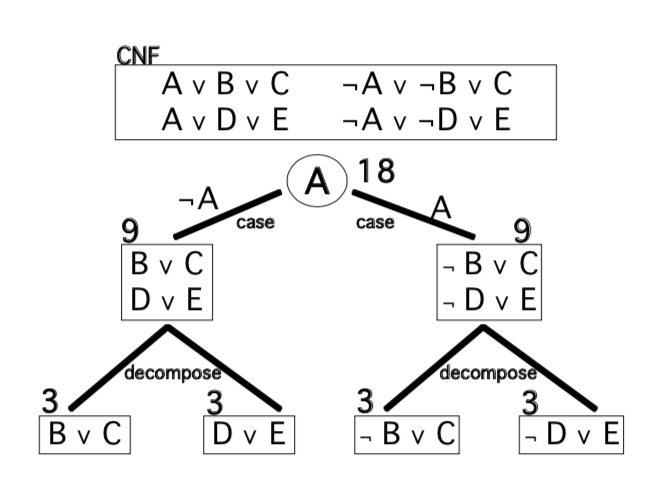
\includegraphics[width = 0.5 \textwidth]{pic/searchalgo.png}
        \caption{The illustration of search based algorithm to perform model counting from \cite{2008-literature-review}}
        \label{fig:searchfig}
    \end{figure}
    
   \noindent  Compared to the Compile-based model counters, model counters by searching require less computational space. One of the most widely search\-based model counter is called cachet proposed in \cite{Cachet}, combined with the encoding method we discussed in 1.2.5 Cachet Encoding, it showed strong ability to perform probabilistic inference and the result was demonstrated in \cite{Sang:2005:PBI:1619332.1619409}\\
    
    \noindent \textbf{SharpSAT:}\\
    Similar to Cachet, the SharpSAT first proposed in \cite{Sharp-SAT2006} used the DPLL algorithm. SharpSAT model counter improved the performance using techniques such as Component Caching and cache management. Compared to Cachet, SharpSAT make use of implicit Boolean constain propogation that result in smaller search space to save the cache space.
    
    \subsubsection{Compile based model counter}
    Another categrory of model counter use knowledge compilation, which the process aims to compile one type logic form into another one.\cite{2008-literature-review} In \cite{2002language-map}, a \textit{represented language} (such as CNF) is defined as sth we expect human to read and write without too much effort, and the \textit{target compilation langauge} are in the form such that it can repond queried in poly\-time. Some of the widely used compile\-based model counters are C2D and miniC2D.\\
    
    \noindent \textbf{C2D}:\\
    C2d was deveploped by UCLA Reasoning group. In \cite{c2d}, the CNF of a Bayesian network, encoded using Full Encoding discussed above, was compiled in to d\-DNNF, and this is a form of knowledge representation knowledge that support model counitng in poly\-time to the size of the input compiled form (d\-DNNF) \cite{2002language-map}.\\
    
    \noindent Model counting require three property, decomposition, determinism, and smoothness which is satisfied by d\-DNNF. Compiling CNF into d\-DNNF will support weighted model counting by traversing the d\-DNNF and multiply or add the results.\\
    
    \noindent \textbf{mini-C2D}:\\
    \noindent The model counter mini\-C2D was proposed in \cite{minic2d}. Minic2d is a top\-down compiler that given the CNF clauses as input, it compile the CNF into Sentential Decision Diagram (SDD).\\
    
   \noindent One of the main disadvantages is that the compiled file size can be larger than the available memory, futher results are shown in the Results and analysis in Section 7.6.
    
    \subsection{Selection and decision}
    In this project, we implemented the encoding schemes including Full encoding, Simplified Full encoding, Improved encoding and Group encoding, and I used the miniC2D for model counting. \\
    
    \noindent The four encoding schemes are closely related to each other and perform improvement step by step. Thus, it is more fair to compare the performance during the model counting phase.\\
    
    \noindent The model counting tool is miniC2D. We chose miniC2D because it is a cross platform software package that support both MacOS and Linux. The weight is formatted in a simpler way in one line compared to other available model counters. In addition, according to \cite{minic2d}, the performance is among the best.\\
    
    \noindent In \cite{2008-literature-review}, the combining of the four encoding schemes and compiled based model counters give strong performance and good results. It is reasonable to expect the newer model counter miniC2D can perform equally strong for the benchmark problems.
    
    % \subsubsection{Cachet and C2D model counter}
    % Cachet is a search based model counter \cite{Cachet}. The idea behind is to decompose the CNF clauses into several components that does not share variables, so that each component can be counted separately. When all the clauses share some same variables, splitting is required to force the decomposition. \\\par
    % Compared to some of the model counter that explore  topological structure, Cachet performed better in the experiment in \cite{2008}.\\\par
    % C2D \cite{c2d} is a knowledge compiler that is based on a search based model counter, while it keep trace of its operations, and it also use a different method to implement decomposition, variable splitting and caching.
    % \subsubsection{Ace model counter}
    % Ace \cite{Ace} is a knowledge compilation based model counter that compile one logical form into another target logical form. For example, in section 2.1.1, after encoding the Bayesian Networks into CNF using Encoding 1, The CNF need to be compiled into d-DNNF. The d-DNNF supports model counting in polytime in the size of the compiled form.
    
